\documentclass{article}

\usepackage{amsmath}
\usepackage{amssymb}
\usepackage{mathtools}
\usepackage{fullpage}
\usepackage{enumerate}
\usepackage{graphicx}

\title{Computer Science 577 Notes \\ Machine Learning}
\author{Mendel C. Mayr}
\date{\today}

\begin{document}
	\maketitle
	\vspace{10pt}
	\begin{center}
		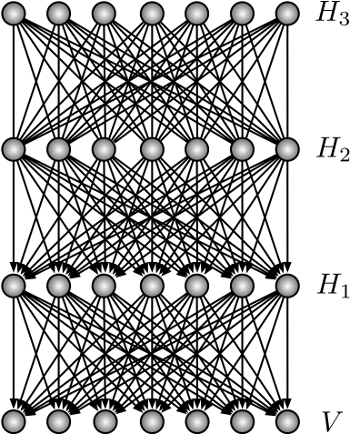
\includegraphics[width = 2.9in]{ann.png}
		\end{center}
	\vspace{16pt}
	\tableofcontents
	\clearpage

	\section{Decision Tree Learning}
		Information gain is used to determine the (feature to) split \\
		Information theory: entropy and information gain:
		\begin{enumerate}[(i)]
			\item Entropy $= H(X) = -\sum_{x \in X}P(X = x)\log_2 P(X = x)$
			\item Conditional entropy $= H(Y|X) = -\sum_{x \in X}P(Y|X = x)$, where \\
			$H(Y|X = x) = \sum_{y \ in Y}P(Y = y|X = x)\log_2 P(Y = y|X = x)$
			\item Mutual information (information gain) $= I(X, Y) = H(Y) - H(Y|X)$
			\end{enumerate}
		Alternative metric: Gini coefficient, i.e. product of probabilities for each of (2) outcomes for the feature \\
		\\
		Limitation of information gain: biased toward tests with many outcomes (i.e. features with many possible values) \\
		C4.5 uses gain ratio: $SplitInfo(D, S) = -\sum_{k \in S} |D_k|/|D| log_2(D_k/D)$, and $GainRatio = I(D, S)/SplitInfo(D, S)$ \\
		\\
		Overfitting: $h \in H$ overfits the training data $D$ if there is an alternative model $h' \in H$ such that $error(h) > error(h')$ yet $error_D(h) < error_D(h)$ \\
		Avoiding overfitting in decision tree learning:
		\begin{enumerate}[(i)]
			\item Early stopping: stop if further splitting not justified by statistical test
			\item Post-pruning: grow large tree, then prune nodes using tuning set \\
			Iteratively eliminate nodes until further reductions reduce accuracy
			\end{enumerate}
		Lookahead: instead of evaluating using information gain, look ahead to see what splits at the next level would be, and measure information gain at a deeper level \\
		\\
		Continuous features: use threshold-based boolean attribute, treshold determined by sorting examples according to the featurem and generating candidate thresholds between adjacent examples with different class values \\
		Threshold chosen from candidates based on information gain \\
		\\
		Training examples with missing attribute values: possible strategies
		\begin{enumerate}[(i)]
			\item At node $n$, upon encountering a missing feature value, assign it the value most common among examples at node $n$, or most common among examples at the node $n$ that also have the same class value
			\item Assign fractional value to attribute for the example and pass fractional example to children for purposes of evaluating information gain
			\end{enumerate}
		\clearpage

	\section{Instance-Based Learning}
		$k$-nearest neighbor classification: given an instance $x_q$ to classify, find $k$ training-set instances that are most simimlar or $x_q$ \\
		Return the class value: $\hat{y} = argmax_{v \in values(Y)} \sum_{i = 1}^k \delta(v, y_i)$ \\
		Various determinations of distance: 
		\begin{enumerate}[(i)]
			\item Hamming distance: number of features with differing values
			\item Euclidean distance: $\delta(x_i, x_j) = \sqrt{\sum_f ({x_i}_f - {x_j}_f)^2}$
			\item Manhattan distance: $\delta(x_i, x_j) = \sum_f ({x_i}_f - {x_j}_f)^2$
			\end{enumerate}
		$k$-nearest neighbor regression: given an instance $x_q$, find the $k$ nearest training-set instances and return $\sum_{i = 1}^k \delta(v, y_i)$ \\
		Distance-weighted nearest neighbor: instances contribute to prediction according to their distance from $x_q$ \\
		\\
		$k$-nearest neighbor does almost nothing at training time, and offsets costs to classification/prediction time \\
		Strategies to speed up $k$-nearest neighbor
		\begin{enumerate}[(i)]
			\item Don't retain every training instance: edited nearest neighbor \\
			Select subset of instances that still provide accurate classifications: \\
			\begin{enumerate}[(a)]
				\item Incremental deletion: delete from memory all training instances redundant to classification
				\item Incremental growth: if training instances insufficient to classify training instance, add to memory
				\end{enumerate}
			\item Use data structure to look up nearest neighbors ($k$-$d$ tree)
			\end{enumerate}
		$k$-$d$ trees ($A^*$ instance search): each node stores one instance, and splits on the median value of the feature having the highest variance \\
		Nodes are pushed to the $A^*$ priority queue with the value indicating the minimum possible distance to the query based on the threshold for the split \\
		\\
		Strenghts of instance based learning: simple, efficeint training, easily adapts to on-line nearning, rubust to noisy data, etc. \\
		Limitations: sensitive to range of feature values, senstivie to irrelevant and correlated features, inefficient classification, no insight into problem domain (i.e. lacks modeling of problem)
		\clearpage

	\section{Probability and Bayesian Learning}
		Recall Bayes theorem: $P(A|B) = P(B|A)P(A)/P(B)$ \\
		\\
		Brute-force MAP learning algorithm:
		\begin{enumerate}[(i)]
			\item Given information $D$, for each hypothesis $h \in H$, calculate the posterior probability $P(h|D) = P(D|h)P(h)/P(D)$
			\item Output hypothesis $h_{MAP}$ with highest posterior probability $h_{MAP} = argmax_{h \in H} P(h|D)$
			\end{enumerate}
		Other probabalisitic methods in machine learning:
		\begin{enumerate}[(i)]
			\item Maximum likelihood and least-squared error hypotheses
			\item Maximum likelihood hypotheses for predicting probabilities
			\item Minimum description length principle
			\item Bayes optimal classification: $argmax_{v_j \in V}\sum_{h_i \in H} P(v_j|h_i)P(h_i|D)$
			\item Gibb's Algorithm: choose hypothesis $h \in H$ at random, according to posterior probaiblity distribution over $H$, and use $h$ to predict the classification of the next instance $x$ \\
			\end{enumerate}
		Bayesian networks and naive classification: \\
		\\
		If the data $D$ is noise free, and the target concept is contained in the hypothesis, every hypothesis consistent with the data \\
		Other probabalistic hypotheses concepts:
		\begin{enumerate}[(i)]
			\item Maximumd likelihood and least-squared error hypotheses
			\end{enumerate}
		A Bayesian network consists of a directed acyclic graph and a set of conditional probability distributions \\
		In the each Directed Acyclic Graph (DAG):
		\begin{enumerate}[(i)]
			\item Each node denotes a random variable
			\item An edge from $X$ to $Y$ represents that $X$ directly influences $Y$
			\item Each node $X$ contains a conditional probability distribution representing $P(X|Parents(X))$
			\item Each variable $X$ is independent of its non-descendants given its parents
			\item Each variable $X$ is independent of all others given its Markov blanket
			\end{enumerate}
		Advantages of Bayesian network representation:
		\begin{enumerate}[(i)]
			\item Captures indepdendence and conditional indpendence where they exist
			\item Encodes the relevant  portion fo the full joint distribution
			\item Graphical representation gives insight into complexity of inference
			\end{enumerate}
		\clearpage

	\section{Machine Learning Methdology}
		\clearpage

	\section{Computational Learning Theory}
		\clearpage

	\section{Ensemble Methods}
		\clearpage

	\section{Neural Networks and Deep Learning}
		\clearpage

	\section{Support Vector Machines}
		\clearpage

	\section{Reinforcement Learning}
		\clearpage
	
	\section{Rule Learning and Inductive Logic Programming}
		\clearpage	

	\section{Statistical Relational Learning}
		\clearpage

	\section{Bias-Variance Tradeoff}
		\clearpage

	\section{Real-Valued Prediciton Methods}
		\clearpage

	\section{Dimensionality Reduction}
		\clearpage

	\appendix


	\end{document}